\documentclass[tikz,border=8pt]{standalone}
\usepackage[T1]{fontenc}
\usepackage[utf8]{inputenc}
\usepackage{lmodern}
\usepackage{xcolor}
\usetikzlibrary{arrows.meta,positioning,fit,shapes.misc}

\definecolor{astblue}{HTML}{DCEEFF}
\definecolor{astgreen}{HTML}{DFF5E1}
\definecolor{astyellow}{HTML}{FFF3CC}
\definecolor{astpink}{HTML}{FBE1EA}
\definecolor{astgray}{HTML}{F4F4F4}
\definecolor{astline}{HTML}{5A6B7A}

\tikzset{
  box/.style={
    draw=astline,
    rounded corners=3pt,
    thick,
    align=left,
    font=\sffamily\small,
    text width=5.0cm,
    inner sep=6pt
  },
  smallbox/.style={
    draw=astline,
    rounded corners=3pt,
    thick,
    align=left,
    font=\sffamily\small,
    text width=4.1cm,
    inner sep=6pt
  },
  title/.style={
    font=\sffamily\bfseries\Large,
    text=black
  },
  arrow/.style={
    -{Latex[length=3mm,width=2mm]},
    thick,
    draw=astline
  },
  note/.style={
    font=\sffamily\footnotesize,
    text=black!75,
    align=left
  }
}

\begin{document}
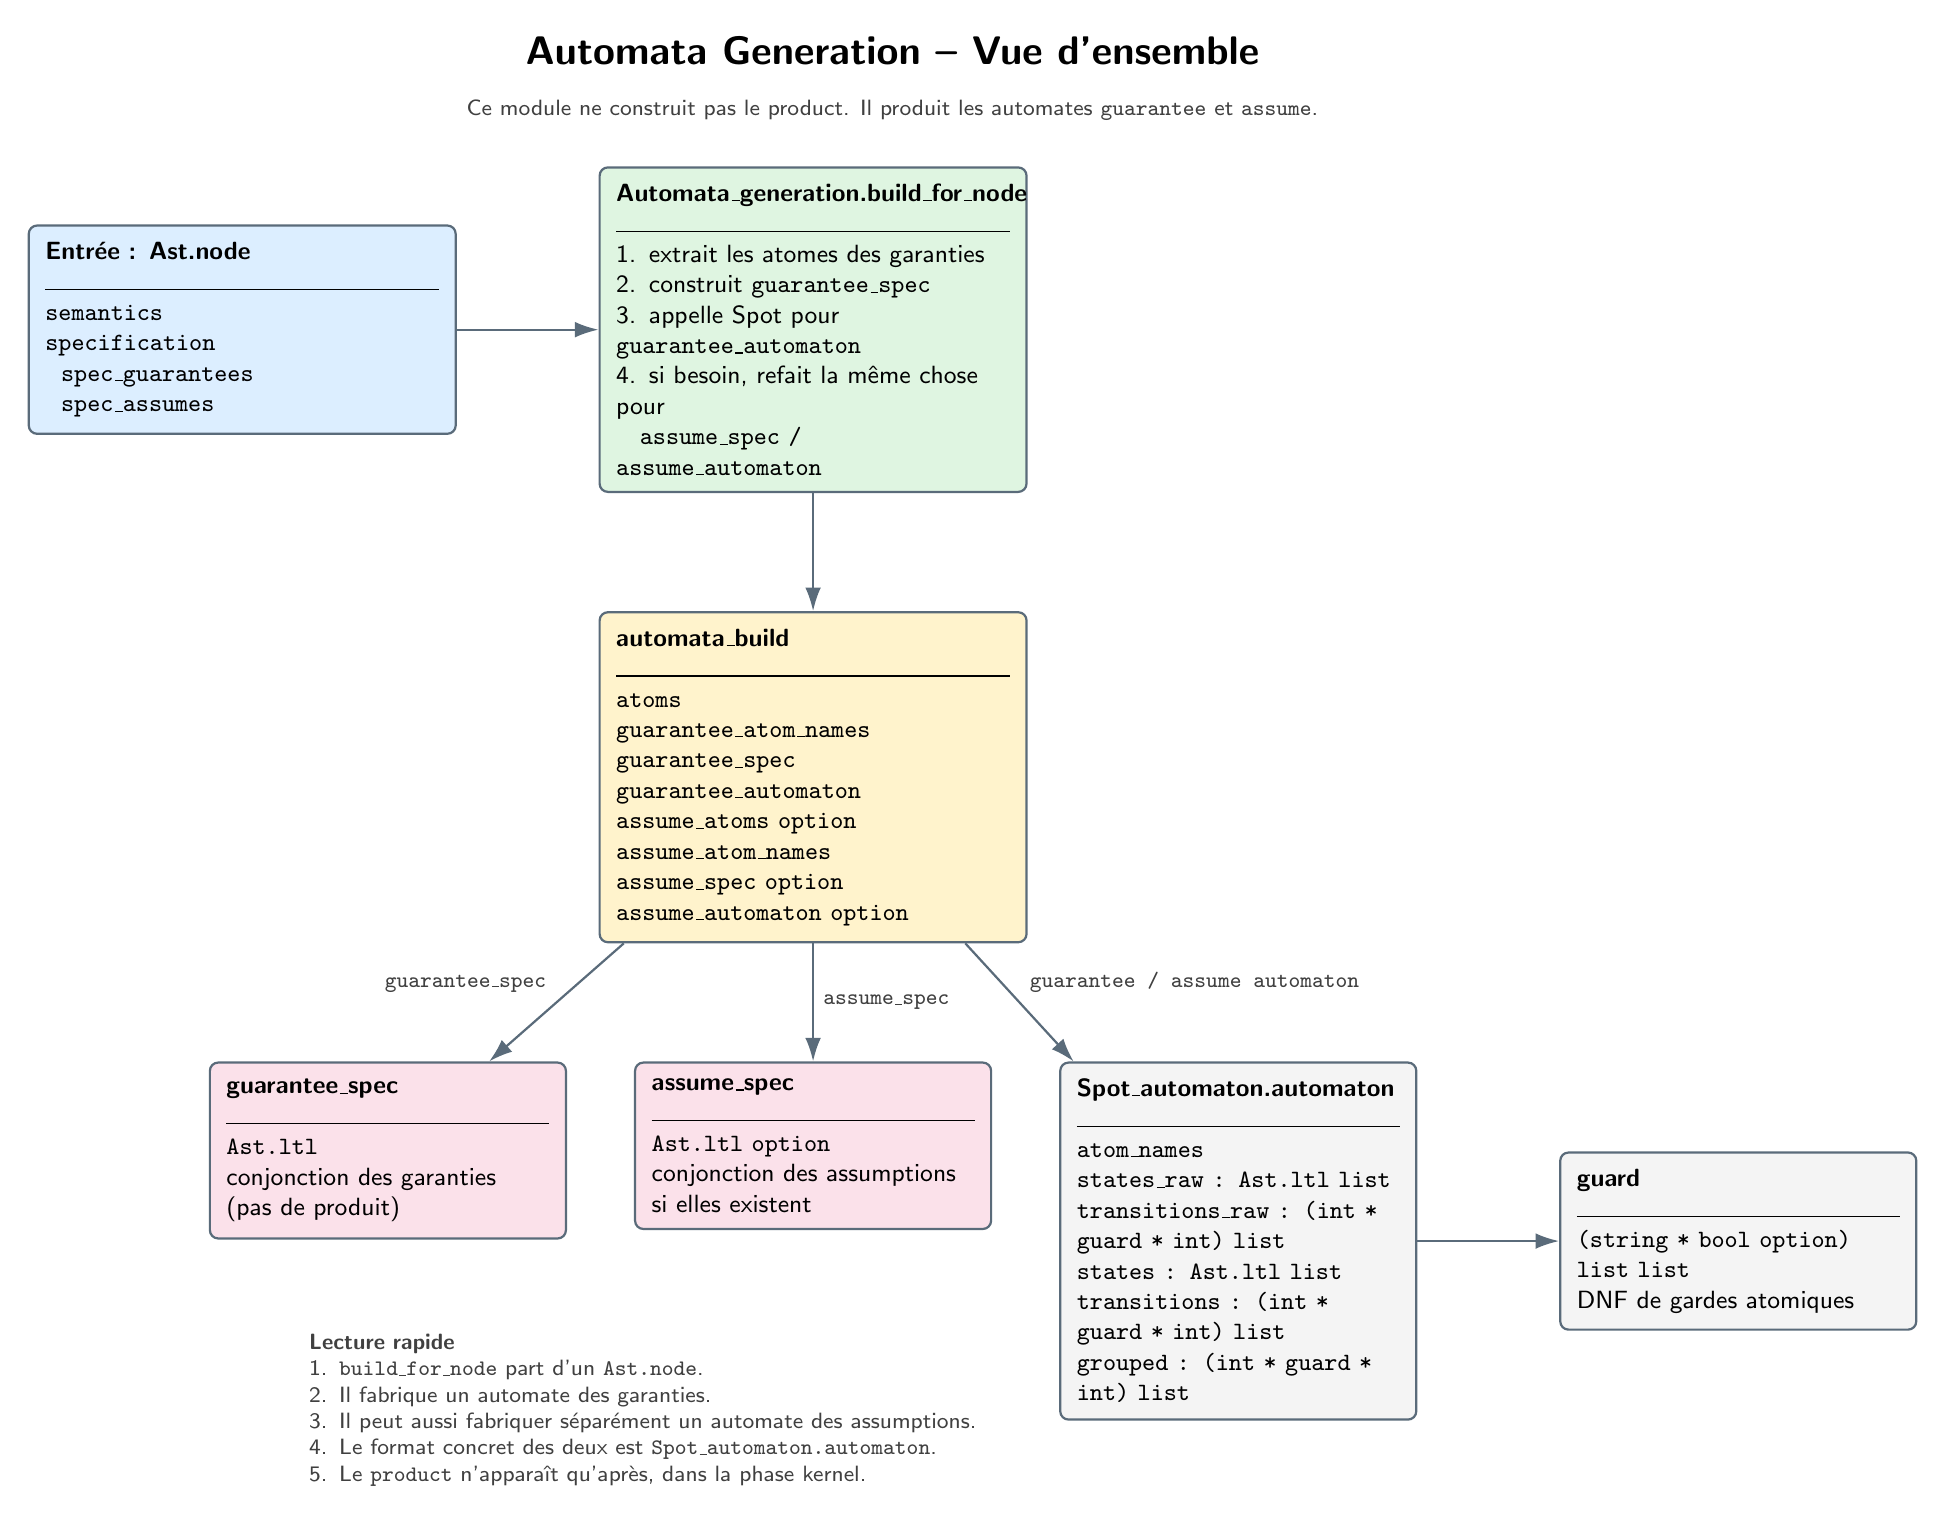
\begin{tikzpicture}[node distance=10mm and 12mm]

\node[title] (title) {Automata Generation -- Vue d'ensemble};
\node[note, below=2mm of title] (subtitle)
  {Ce module ne construit pas le product. Il produit les automates \texttt{guarantee} et \texttt{assume}.};

\node[box, fill=astblue, below left=12mm and 0mm of subtitle] (input) {
  \textbf{Entrée : Ast.node}\\
  \rule{\linewidth}{0.4pt}\\
  \texttt{semantics}\\
  \texttt{specification}\\
  \hspace*{2mm}\texttt{spec\_guarantees}\\
  \hspace*{2mm}\texttt{spec\_assumes}
};

\node[box, fill=astgreen, right=18mm of input] (buildfornode) {
  \textbf{Automata\_generation.build\_for\_node}\\
  \rule{\linewidth}{0.4pt}\\
  1. extrait les atomes des garanties\\
  2. construit \texttt{guarantee\_spec}\\
  3. appelle Spot pour \texttt{guarantee\_automaton}\\
  4. si besoin, refait la même chose pour\\
  \hspace*{3mm}\texttt{assume\_spec / assume\_automaton}
};

\node[box, fill=astyellow, below=15mm of buildfornode] (build) {
  \textbf{automata\_build}\\
  \rule{\linewidth}{0.4pt}\\
  \texttt{atoms}\\
  \texttt{guarantee\_atom\_names}\\
  \texttt{guarantee\_spec}\\
  \texttt{guarantee\_automaton}\\
  \texttt{assume\_atoms option}\\
  \texttt{assume\_atom\_names}\\
  \texttt{assume\_spec option}\\
  \texttt{assume\_automaton option}
};

\node[smallbox, fill=astpink, below left=15mm and 4mm of build] (guarantee) {
  \textbf{guarantee\_spec}\\
  \rule{\linewidth}{0.4pt}\\
  \texttt{Ast.ltl}\\
  conjonction des garanties\\
  (pas de produit)
};

\node[smallbox, fill=astpink, below=15mm of build] (assume) {
  \textbf{assume\_spec}\\
  \rule{\linewidth}{0.4pt}\\
  \texttt{Ast.ltl option}\\
  conjonction des assumptions\\
  si elles existent
};

\node[smallbox, fill=astgray, below right=15mm and 4mm of build] (spot) {
  \textbf{Spot\_automaton.automaton}\\
  \rule{\linewidth}{0.4pt}\\
  \texttt{atom\_names}\\
  \texttt{states\_raw : Ast.ltl list}\\
  \texttt{transitions\_raw : (int * guard * int) list}\\
  \texttt{states : Ast.ltl list}\\
  \texttt{transitions : (int * guard * int) list}\\
  \texttt{grouped : (int * guard * int) list}
};

\node[smallbox, fill=astgray, right=18mm of spot] (guard) {
  \textbf{guard}\\
  \rule{\linewidth}{0.4pt}\\
  \texttt{(string * bool option) list list}\\
  DNF de gardes atomiques
};

\node[note, below=12mm of assume, text width=12.8cm] (legend) {
  \textbf{Lecture rapide}\\
  1. \texttt{build\_for\_node} part d'un \texttt{Ast.node}.\\
  2. Il fabrique un automate des garanties.\\
  3. Il peut aussi fabriquer séparément un automate des assumptions.\\
  4. Le format concret des deux est \texttt{Spot\_automaton.automaton}.\\
  5. Le \texttt{product} n'apparaît qu'après, dans la phase kernel.
};

\draw[arrow] (input) -- (buildfornode);
\draw[arrow] (buildfornode) -- (build);
\draw[arrow] (build) -- node[midway, above left, note] {\texttt{guarantee\_spec}} (guarantee);
\draw[arrow] (build) -- node[midway, right, note] {\texttt{assume\_spec}} (assume);
\draw[arrow] (build) -- node[midway, above right, note] {\texttt{guarantee / assume automaton}} (spot);
\draw[arrow] (spot) -- (guard);

\end{tikzpicture}
\end{document}
